\chapter{Results of Workflow Validation}\label{chap:results}
The developed Galaxy workflows are evaluated using real-world datasets from different laboratories. The analysis results for each workflow with complying test samples are described below.

\section{Poxvirus Workflow with Lumpy Skin Disease Virus Datasets}
We employed the poxvirus pipeline using a tiling amplicon approach with masked reference sequences for each half genome to ensure an unambiguous mapping to the identical two \ac{ITR} regions of the poxvirus genome. Two public \ac{LSDV} samples, 20L70 (MZ577075.1) and 20L81 (MZ577076.1), that were sequenced using a primer scheme with two primer pools, are used and retrieved from GenBank on 10\textsuperscript{th} April, 2023. Collected from cattle  during a lumpy skin disease outbreak in Northern Vietnam in 2020 (20L70\_Dinh-To/VNM/20 and 20L81\_Bang-Thanh/VNM/20), both samples were sequenced on a MiSeq System using a Nextera XT library preparation kit. \\
The used \acs{CaPV} primer scheme in \ac{BED} format contains information about the primer pairs used for the amplicons. Each primer pair has one positive and one negative strand primer, indicated by the strand sign in the sixth column and by the \textit{LEFT} and \textit{RIGHT} label in the name. Amplification of the \ac{PCR} reaction was done in four pools, to denote the two genome halves (\textit{pool1} and \textit{pool2}) and their even and odd numbered amplicons that each have small overlaps and cover the entire genome length. Primers are labeled in an alternating way: \textit{pool1} primer pairs are denoted as \textit{pool1a} (even) and \textit{pool1b} (odd). We use the same method for \textit{pool2} with \textit{pool2a} and \textit{pool2b}. We reuse the \textit{SCORE} column from the \ac{BED} file to unambiguously identify primer and strand for each amplicon. The annotated primer scheme for \ac{CaPV} is part of the workflow run to which links are provided in Supplementary~\secref{sec:apx-aiv-links}. The \ac{LSDV} ``Neethling'' strain, the publicly agreed reference for \ac{LSDV}, was used as reference genome (NC\_003027.1, retrieved from \ac{NCBI} RefSeq on 10\textsuperscript{th} April, 2023) for mapping. The raw FASTQ files for each sample were quality trimmed with \texttt{fastp} and mapped to each half-masked reference, which is explained in detail below. Preprocessing with default \texttt{fastp} settings includes automatically detected adapter trimming, a quality filter to discard reads below an average quality of Q15, with more than 5 uncalled N-bases and 40\% unqualified bases, a length filter to discard reads below a threshold of 30, automatic trimming of polyG tails for Illumina NextSeq/NovaSeq data and a minimum length of 10 to detect polyG tails.
\\

\setlength{\tabcolsep}{16pt}
\renewcommand{\arraystretch}{1.3}
\begin{table}[ht!]
    \centering
    \hspace*{-12pt}
        \begin{tabular}{l|cc|ll}
        \hline
                                                                                           & \multicolumn{2}{c|}{\textbf{Pool1}}                                                                                               & \multicolumn{2}{c}{\textbf{Pool2}}                                                                                                                                        \\ \hline
        \textbf{Output Metric}                                                             & \textbf{\begin{tabular}[c]{@{}c@{}}Sample\\ 20L70\end{tabular}} & \textbf{\begin{tabular}[c]{@{}c@{}}Sample\\ 20L81\end{tabular}} & \multicolumn{1}{c}{\textbf{\begin{tabular}[c]{@{}c@{}}Sample\\20L70\end{tabular}}} & \multicolumn{1}{c}{\textbf{\begin{tabular}[c]{@{}c@{}}Sample\\20L81\end{tabular}}} \\ \hline
        Paired-end raw reads                                                               & 863 820                                                         & 1 016 168                                                       & 862 040                                                                             & 867 440                                                                             \\
        \begin{tabular}[c]{@{}l@{}}Paired-end reads after\\ quality trimming\end{tabular}  & 856 138                                                         & 947 064                                                         & 852 608                                                                             & 819 092                                                                             \\
        \begin{tabular}[c]{@{}l@{}}Proportion of reads\\ mapping to reference\end{tabular} & 99.6\%                                                          & 77.3\%                                                          & 94.1\%                                                                              & 79.3\%                                                                              \\
        Alignment error rate                                                               & 1.25\%                                                          & 1.30\%                                                          & 1.35\%                                                                              & 1.41\%                                                                              \\ \hline
                                                                                           & \multicolumn{2}{c|}{\textbf{Sample 20L70}}                                                                                        & \multicolumn{2}{c}{\textbf{Sample 20L81}}                                                                                                                                 \\ \hline
        Mean coverage                                                                      & \multicolumn{2}{c|}{{2 705.2\texttimes }}                                                                                                      & \multicolumn{2}{c}{{2 411.4\texttimes }}                                                                                                                                               \\
        \begin{tabular}[c]{@{}l@{}}Proportion of reference\\ covered\end{tabular}          & \multicolumn{2}{c|}{99.68\%}                                                                                                      & \multicolumn{2}{c}{99.68\%}                                                                                                                                               \\ \hline
    \end{tabular}
    \caption[Metrics after preprocessing and mapping for datasets 20L70 and 20L81.]{Metrics after preprocessing and mapping for datasets 20L70 and 20L81 divided by pools.}
\label{tab:4-pox-metrics}
\end{table}

The used primer scheme contains a total of 23 primers, while the first set of primers 1 to 12 covers the 5' genome end labeled with \textit{pool1}, and the remaining 11 primers (13 to 23) cover the 3' genome end, labeled with \textit{pool2} as depicted at the top in blue (\textit{pool1}) and red (\textit{pool2}) in~\figref{fig:3-pox-ampl}. This scheme was designed for the tiling amplicon approach all three members of Capripoxviruses, which includes the \ac{LSDV} samples. To use the primer scheme with \ac{SPPV} or \ac{GTPV} samples and to account for the shorter genome lengths, the primer positions need to be shifted to the correct coordinates.\\
The used primer scheme is provided in the Galaxy history of the test runs and is available via links in Supplementary~\secref{sec:apx-pox-links}. Inspection of the masking boundaries for N-masking the reference confirms that the right-most position of masking the 5' half (i.e. preparing the reference for mapping \textit{pool2} reads) is the minimal start position of \textit{pool2} primers (``1 -- 79081'', and 79081 being the start position of primer 13). Accordingly for N-masking the reference for mapping of \textit{pool1} reads, the position of the right-most primer end of \textit{pool1} primers (primer 12) is 80202, resulting in the interval ``80202 -- 150773''. \ac{BED} files are 0-based, meaning that the first named position is the first base of the given interval, and the last position is the first base outside the interval in the \ac{BED} file. The overlapping merging region in the middle of the genome is clearly visible in~\figref{fig:4-lsdv-read-groups}, where reads from \textit{pool1} are labeled in red and \textit{pool2} in blue, and mapped to the same reference sequence with different masked parts. 
\begin{figure}[ht!]
    \centering
    \hspace*{-24pt}
    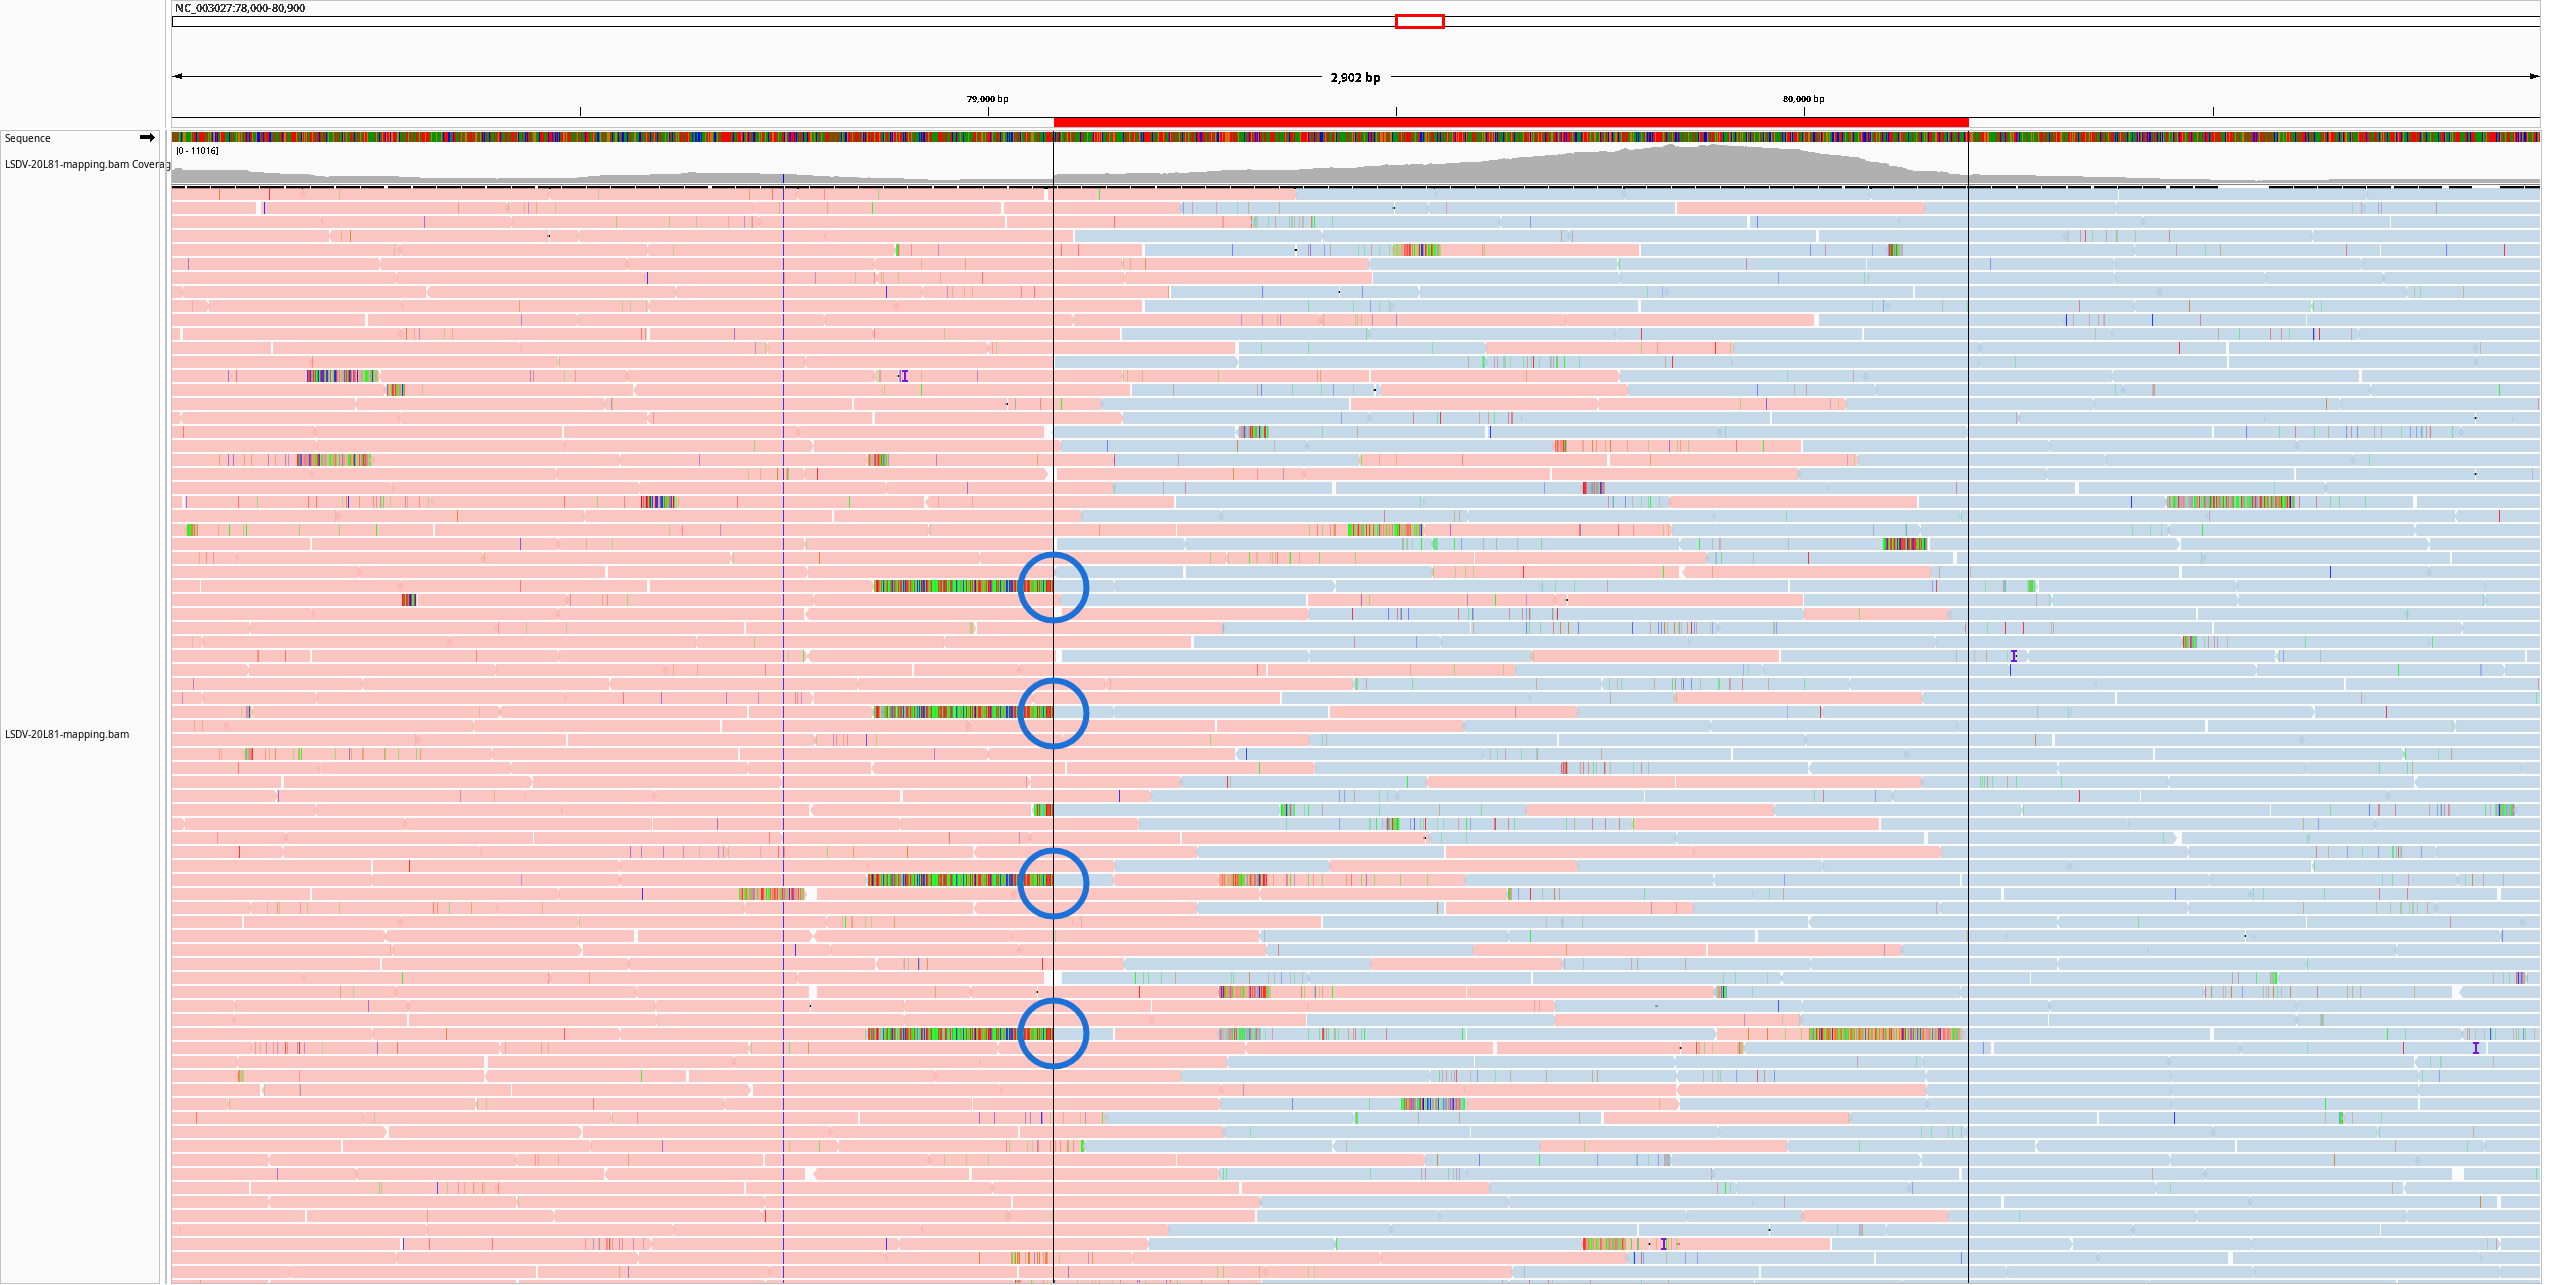
\includegraphics[width=1.1\textwidth]{media/4-lsdv-alig-20L81-c.png}
    \caption[Overlapping reads region of LSDV mapping in 20L81 sample.]{Overlapping, seamlessly merged mapping region of the two amplicon pools of the 20L81 sample. Coloured reads indicate read groups from \textit{pool1} (red) and \textit{pool2} (blue), primers are soft-clipped and end where the mapping of \textit{pool2} reads starts, as marked with blue circles for primer 13 to which four reads from \textit{pool2} bind. More primers may bind outside of the cropped snapshot.}
    \label{fig:4-lsdv-read-groups}
\end{figure}

Since the reference genome and primer scheme are the same for both datasets 20L70 and 20L81, the N-masked references are used for both mappings in a multisample workflow run. Mapping of each pool is done with \texttt{BWA-MEM} and default settings for Illumina-sequenced reads, using the N-masked reference for \textit{pool1} and \textit{pool2} respectively. This results in a mapping with a small overlap in the central part of the genome, where primer 12 ends and primer 13 starts as indicated in the top of~\figref{fig:3-pox-ampl}. It has a length of 1,121 bases. After merging the mappings with \texttt{Samtools merge}, statistics for preprocessing and mapping are reported and summarised in~\tabref{tab:4-pox-metrics}. It shows that the samples yield similarly good quality mappings with error rates during the alignment of a maximum of 1.41\%. The 20L70 sample has a larger share of reads that map to the reference (99.6\% of \textit{pool1} and 94.1\% of \textit{pool2} sequenced reads), although its absolute amount of reads is larger at least in \textit{pool1}.\\
\figref{fig:4-lsdv-read-groups} shows a snapshot from \ac{IGV}, where the mappings of \textit{pool1} reads (red) and \textit{pool2} reads (blue) are merged and clearly complement each other. They demonstrate a higher coverage in the overlapping part of the reference which was mapped to in both pools, with peaking values of circa {13 800\texttimes }. For both samples 20L70 and 20L81, almost the complete reference genome was covered during mapping (99.68\%) with a mean coverage of {2705.2\texttimes } and {2411.4\texttimes } respectively. There are very few minimums where coverage drops to under {500\texttimes }. Primer end positions of \textit{pool2} primers are highlighted with blue circles and mark the start position of the overlapping region and the end of the masking of the reference sequence for \textit{pool2}. According to a graph for mapping quality across the reference, mapping quality has high values of circa Q60, except for one outstanding minimum at around position 118,000 of the reference. This occurs in both of the test samples.\\
The merged mapping of both read pools was quality trimmed with \texttt{iVar trim} to mask primers and mapped reads with a length of less than 30 bp, so they are excluded during consensus construction. The remaining reads were used for full-length consensus sequence construction with \textit{iVar consensus}, developed for amplicon-based sequencing data. Inspection of the consensus sequences for both samples shows that apart from low coverage regions in the 5' front and 3' tail due to ampliconic sequencing, a consensus sequence was produced and a base at each position could be found. A base could not be called in the consensus at the first 264 positions in both the 20L70 and 20L81 sample, which corresponds to the primer binding site on the forward strand, and no bases at the last 268 positions indicate the remaining part where the last primer on the reverse strand starts. This was expected due to ampliconic sequencing where the first primer ends at genomic position 264, and where the target sequence starts. In the 3' end, the trailing Ns start at position 150,505, which is exactly the last position outside the primer (Primer 23 on the reverse strand, \textit{pool2a}), which starts at position 150,505. All in all, this means that the maximum consensus sequence was found between the first and the last primers. The workflow ends by producing a collection of the per-sample consensus sequences.

\subsubsection*{Poxvirus Workflow Validation using other CaPV Reference Sequences}
Until 2017, genomic analysis of different \ac{LSDV} samples from all over the world suggested very limited genomic variation. There are two phylogenetic clusters that were thought to be stable: the Neethling-based strain (used for vaccine development) and a wild-type strain~\cite{biswas2020extended}. In 2018, a report has been filed from a vaccine-like field isolate that revealed the presence of multiple recombination sites within the sample while one of the found parental strains was the Neethling vaccine strain (referred to as Saratov strain as in~\secref{sec:2-pox})~\cite{sprygin2018analysis}. Following current sequencing efforts, the existence of more recombinant clusters has been demonstrated from field isolates that took the Neethling-based vaccine. Analysis of this vaccine revealed the presence of multiple Capripoxviruses within the sample: the Neethling-vaccine strain, a KSGP-based vaccine strain, a \ac{GTPV} strain from Sudan and most importantly other different recombinants between KSGP and Neethling strains. These studies suggest that this recombinant \ac{LSDV} strain that currently spreads in Asia is likely caused by a vaccine spillover~\cite{vandenbussche2022recombinant}. The Kenyan Sheep and Goat Pox (KSGP) strain was first detected in \ac{LSDV}-infected sheep and goats from Kenya, although it has been used for sheeppox and goatpox vaccines~\cite{tuppurainen2014characterization}. The Vietnamese test samples 20L70 and 20L81 are shown to be recombinant with these two parent strains~\cite{vandenbussche2022recombinant}.

\setlength{\tabcolsep}{8pt}
\renewcommand{\arraystretch}{1.3}
\hspace*{-24pt}
\begin{table}[ht!]
    \centering
    \begin{tabular}{@{}lccccc@{}}
    \toprule
                            & \multicolumn{1}{l}{\textbf{\begin{tabular}[c]{@{}l@{}}LSDV-\\ Neethling\end{tabular}}} & \multicolumn{1}{l}{\textbf{\begin{tabular}[c]{@{}l@{}}LSDV-\\ KSGP\end{tabular}}} & \multicolumn{1}{l}{\textbf{\begin{tabular}[c]{@{}l@{}}LSDV-\\ Herbivac\end{tabular}}} & \multicolumn{1}{l}{\textbf{SPPV}} & \multicolumn{1}{l}{\textbf{GTPV}} \\ \midrule
    \textbf{\begin{tabular}[c]{@{}l@{}}LSDV-Neethling\\\textnormal{(NC\_003027.1)}\end{tabular}} & 0                                                                                      & 0.0006                                                                            & 1.1                                                                                   & 2.1                               & 1.8                               \\
    \textbf{\begin{tabular}[c]{@{}l@{}}LSDV-KSGP\\\textnormal{(KX683219.1)}\end{tabular}}      &                                                                                        & 0                                                                                 & 1.1                                                                                   & 2.1                               & 1.8                               \\
    \textbf{\begin{tabular}[c]{@{}l@{}}LSDV-Herbivac\\\textnormal{(KX764644.1)}\end{tabular}}  &                                                                                        &                                                                                   & 0                                                                                     & 2.1                               & 1.9                               \\
    \textbf{\begin{tabular}[c]{@{}l@{}}SPPV\\\textnormal{(NC\_004002.1)}\end{tabular}}           &                                                                                        &                                                                                   &                                                                                       & 0                                 & 2.4                               \\
    \textbf{\begin{tabular}[c]{@{}l@{}}GTPV\\\textnormal{(NC\_004003.1)}\end{tabular}}           &                                                                                        &                                                                                   &                                                                                       &                                   & 0                                 \\ \bottomrule
    \end{tabular}
    \caption[Maximum Likelihood Distance matrix of CaPV strains.]{Distance Matrix based on a maximum likelihood criterion of all clades within the CaPV genus. The LSDV clades are more closely related with each other than SPPV and GTPV, while the LSDV Neethling and KSGP strains are almost identical, and the recombinant LSDV-Herbivac vaccine strain is distinct.}
\label{tab:4-capv}
\end{table}

To determine relations among the strains, a distance matrix (\tabref{tab:4-capv}) was generated which shows the four different known clades within the Capripoxvirus genus. While the \ac{LSDV}-Neethling and KSGP strains are very closely related, the recombinant \ac{LSDV}-vaccine strain differs from this clade. \ac{SPPV} and \ac{GTPV} clades are shown to be more different to the \ac{LSDV} clades. By creating a \ac{MSA} of the reference used for mapping of test sample reads, the constructed consensus sequences and the \ac{LSDV}-vaccine reference (Herbivac, GenBank: KX764644.1, retrieved on 23\textsuperscript{rd} April, 2023), and converting it to a \ac{VCF} file it is possible to detect the patterns of variation found in the published article by Vandenbussche et al, 2022~\cite{vandenbussche2022recombinant}. The tool \texttt{faToVcf} was XML-wrapped as part of this work to make it accessible from within Galaxy. The tool was initially published by the University of California, Santa Cruz (UCSC) and generates a \ac{VCF} file that holds information about single-nucleotide substitutions. Although the \texttt{faToVcf} tool is not capable of displaying indels, it clearly shows unmapped regions in the consensus sequences from the \ac{MSA}. The pattern confirms the findings of the experiments by Vandenbussche et al. by showing a complementing pattern of similarities and differences between the two parental strains, the \ac{LSDV} Neethling strain which is closely related to the KSGP clade, and the \ac{LSDV}-Herbivac clade.
\begin{figure}[ht!]
	\centering
	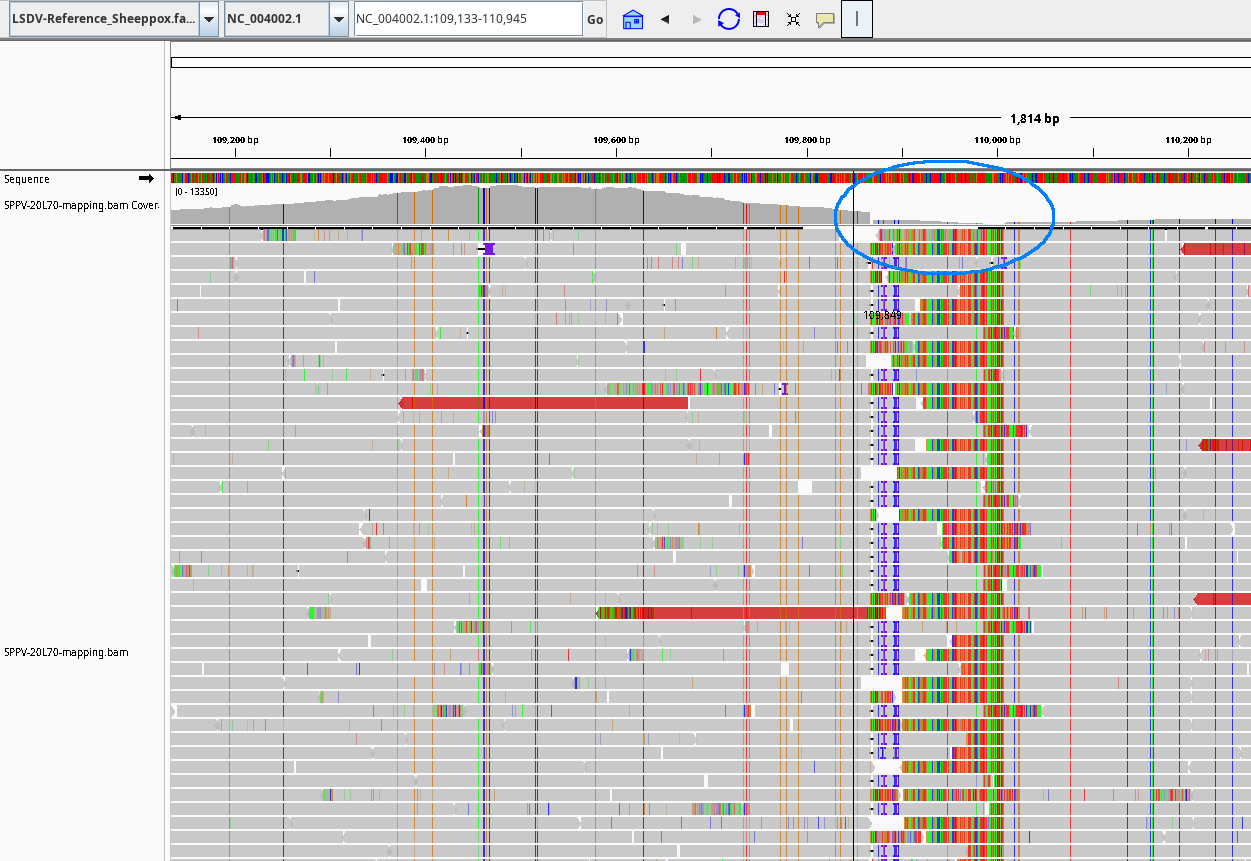
\includegraphics[width=1\textwidth]{media/4-capv-sppv-110.png}
	\caption[Mapping of read ends and primers to incorrect SPPV reference of LSDV reads.]{Mapping of read ends and primers to the incorrect SPPV reference, resulting in low coverage regions.}
	\label{fig:4-capv-sppv-110}
\end{figure}

Discussing \ac{LSDV} strains and clades within the Capripoxvirus genus, the poxvirus workflow for which the test samples were chosen exemplatory, requires a reference for mapping. Since the choice of reference impacts the alignment and subsequent consensus calling, we aim to show that despite the different \ac{CaPV} strains, the choice of reference sequence is not substantial and by knowing the ambiguous genome regions, the clade can be determined. Thus, we started the poxvirus workflow with reference sequences from all four strains (\ac{LSDV}-Neethling: NC\_003027.1; \ac{LSDV}-Herbivac (Neethling-vaccine): KX764644.1; SPPV: NC\_004002.1; \ac{GTPV}: NC\_004003.1, all retrieved from GenBank on 23\textsuperscript{rd} April, 2023) and compare the consensus sequences with their parental strains. The resulting consensus sequences demonstrate few specific locations with ambiguous bases. These are listed, combined with the used reference, in~\tabref{tab:apx-capv-n}. To determine the reasons for ambiguity, i.e. N masking in the consensus, the consensus sequences were aligned to the reference sequence and the \ac{LSDV}-Neethling strain using \texttt{\acs{MAFFT}}. There were ambiguous sites masked with N bases in each of the \texttt{iVar consensus}-generated consensus sequences. The exact positions are listed in Supplementary~\tabref{tab:apx-capv-n} and are highly similar among the two \ac{LSDV} test samples. The list includes Ns that are expected due to ampliconic sequencing as explained above (no. 1, 3, 4, 8, 9, 11).\\
The sample reads are known to be from an \ac{LSDV} strain, and since its reference genome is larger than that of the other \acs{CaPV} members, mapping of the reads to a shorter genome could work for most regions but end in unmapped read ends, that do not fit to the incorrect reference genome. In these indel regions, low coverage leads to ambiguous sites in the consensus sequence. A \ac{MSA} of the consensus sequence, the used reference and the more similar Neethling reference helps to identify such low coverage regions. One location of the consensus sequence mapped to the sheeppox reference, having Ns in genomic positions 110,083--110,106 in the 20L81 sample, is depicted with its mapped reads and suboptimally mapped primer ends in~\figref{fig:4-capv-sppv-110}. It clearly shows that coverage around the 23 nucleotides long region is high, since reads could be mapped to the very similar \ac{SPPV} reference, and immediately drops for the masked region. Another location with a similar pattern occurs in 18,479--18,498 of the consensus sequence (no. 5 in Supplementary~\tabref{tab:apx-capv-n}) based on mapped reads to the \ac{SPPV} reference genome. Regarding ambiguous site no. 2, mapped to a reference of the \ac{LSDV} Herbivac vaccine strain, the length of the masked stretch is constituted of 43 bases explained by sample-specific low coverage region, and 72 bases that are unable to map to the Herbivac strain. This is consistent with the finding from the original article by Vandenbussche et al. (2022), where reads of the 20L81 and 20L70 samples in this region show high genetic variation compared to the parental \ac{LSDV} originating Herbivac genome.\\
The impact of the found point mutations in the \ac{LSDV} test samples was not examined because a gene annotation file for poxviruses with genomic features on the amino acid layer was not available.

\section{AIV Workflow with H4N6 and H5N8 Samples}\label{sec:4-aiv}
\setlength{\tabcolsep}{14pt}
\renewcommand{\arraystretch}{1.3}
\begin{table}[ht!]
    \centering
    \begin{tabular}{lcc} 
    \toprule
    \textbf{Output Metric}                                                                & \textbf{H4N6} & \textbf{H5N8} \\ \midrule
    Paired-end raw reads                                                                  & 1 537 722                  & 858 610                    \\ 
    \begin{tabular}[c]{@{}l@{}}Paired-end reads after quality\\trimming\end{tabular}      & 1 507 396                  & 830 176                    \\ \bottomrule
    \end{tabular}
    \caption[Metrics after preprocessing of H4N6 and H5N8 samples.]{Metrics about Illumina reads before and after preprocessing of H4N6 and H5N8 samples.}
    \label{tab:4-aiv-metrics}
\end{table}

The \ac{AIV} Illumina workflow on the Galaxy platform was evaluated using two field isolates provided by Sciensano, the Belgian national health institute. The isolates were extracted in Belgium in 2020 from an H4N6 infected magpie (EPI\_ISL\_7593059) and an H5N8 infected duck (EPI\_ISL\_7596571). For reasons of readability, we refer to the samples as H4N6 and H5N8 samples. The two samples were sequenced on an Illumina platform in paired-end mode and are utilised one sample per workflow run on Galaxy. For the \ac{AIV} Illumina workflow, a reference database in FASTA format is required as a collection, i.e. a list of one dataset per \ac{AIV} segment, which is uploaded in Galaxy. The used database contains multiple sequences per segment as described in~\secref{sec:3-aiv-ref}. The amount of sequences and distribution of subtypes within each segments suggests that variation within each subtype is generally captured well with the given database.\\
After starting the workflow, the paired-end reads were preprocessed and serve as query reads for \texttt{VAPOR}. Metrics of before and after preprocessing are shown in~\tabref{tab:4-aiv-metrics} and count more than 1.50 million reads after preprocessing for the H4N6 sample and 0.83 million reads for the H5N8 dataset. Since the reference database contains eight FASTA files in a collection, \texttt{VAPOR} runs once per dataset and outputs the highest scoring sequences per segment, which represents the most similar sequences from the database compared to the query sequences. \\

\setlength{\tabcolsep}{8pt}
\renewcommand{\arraystretch}{1.3}
\begin{table}[ht!]
    \centering
    \hspace*{-16pt}
    \begin{tabular}{@{}lcccc@{}}
    \toprule
    \multicolumn{1}{l}{\textbf{Segment}} & \multicolumn{2}{c}{\textbf{Proportion of query bases in reads}}                             & \multicolumn{2}{c}{\textbf{AIV subtype of hit}}                                         \\ \midrule
                                         & \multicolumn{1}{l}{\textbf{H4N6 sample}} & \multicolumn{1}{l}{\textbf{H5N8 sample}} & \multicolumn{1}{l}{\textbf{H4N6 sample}} & \multicolumn{1}{l}{\textbf{H5N8 sample}} \\ \cmidrule(l){2-5} 
    HA                                   & 98.7\%                                    & 100.0\%                                      & H4                                       & H5                                       \\
    NA                                   & 98.7\%                                    & 100.0\%                                      & N6                                       & N8                                       \\ \bottomrule
    \end{tabular}
    \caption[Results of VAPOR run with AIV test samples.]{The best scoring sequence of the VAPOR run for each AIV test samples, indicating a perfect match (100\% of the query bases are in the reads) of the HA and NA segments of the H5N8 sample sequence, and almost all query bases of the H4N6 sample in the found sequemce.}    
\label{tab:4-aiv-vapor}
\end{table}

The \texttt{VAPOR} search was able to successfully identify the avian influenza virus subtypes present in each sample: for the H5N8 sample, the most similar sequence of \ac{HA} segment origins from a sample with the H5 subtype, while the most similar sequence of the \ac{NA} segment origins from a sample with the N8 subtype. Both found gene sequences contain 100\% of the input reads. Similarly, the H4N6 sample was correctly identified with concordance of query bases of 98.7\% each. The results of the \texttt{VAPOR} run for the \ac{HA} and \ac{NA} genes are summarised in~\tabref{tab:4-aiv-vapor}. \\
Consensus sequences for each genome segment were constructed with \texttt{iVar consensus} and while a consensus could be found at each position, the produced consensus sequences are 100\% identical to the originally assembled reads that were uploaded to \ac{GISAID} by the Sciensano laboratory from the same sample (EPI\_ISL\_7593059 and EPI\_ISL\_7596571). Due to slightly different genome sizes of the reference sequence used for mapping compared to the assembly, the resulting consensus sequences in the \ac{AIV} workflow are shorter than the assembled sequences on \ac{GISAID}. The consensus sequence for the \ac{HA} segment of the H4N6 sample is differing in 1 bp in the 5' end, and 4 bp in the 3' end. The consensus sequence constructed for the \ac{NA} gene misses 18 bp compared to the assembled sequence on \ac{GISAID} in the 5' end and 33 bp in the 3' end. Similarily, the \ac{HA} consensus sequence of sample H5N8 is 28 bp shorter in the front and 44 bp shorter in the end. The \ac{NA} consensus sequence differs in 20 and 28 bp in the front and tail. These differences indicate the missing \acp{UTR} on the whole-length genome. While the hybrid reference that was compiled from the eight influenza segments contains complete segments including start and stop codons, which is a criterion for each sequence to be part of the reference database, the aligned consensus sequence does not contain the \acp{UTR} at the 5' and 3' ends as opposed to the \textit{de novo} assembled sequences uploaded to \ac{GISAID}. This was validated by running the \texttt{getorf} tool in Galaxy and reporting the \acp{ORF} as nucleotide sequences between start and stop codons. This analysis showed the presence of full \acp{ORF} in each segment in both test samples.\\
Other workflow outputs for the \ac{AIV} samples include plots that visually emphasise \acp{SNP} relative to the top hits of the \texttt{VAPOR} run, indicating the most similar sequences from the reference collection. The plots for the \ac{HA} and \ac{NA} genes for the H4N6 sample (\figref{fig:apx-aiv-snipit-s4}) show 30 \acp{SNP} compared to the first sequence which was also used as reference for mapping (LC121412.1) and 31 \acp{SNP} compared to the second best result (MK192399.1). Similarly, the \ac{NA} gene consensus sequence has 29 \acp{SNP} compared to the most similar reference sequence (MW19994.1). For the H5N8 sample, the \texttt{VAPOR} run found a sequence with 100\% of the query bases in the reads, and therefore the number of \acp{SNP} was expected to be low. Supplementary~\figref{fig:apx-aiv-snipit-s8} shows there is one \ac{SNP} in the \ac{HA} gene compared to the reference (MZ166252.1) at position 1002 and one \ac{SNP} at position 497 compared to the \ac{NA} reference sequence (MZ166270.1). The \acp{SNP} indicate point mutations or mapping errors, low coverage or close calls during consensus sequence construction. \\
A protein FASTA file containing gene annotations is generated based on the consensus sequence with \texttt{Prokka} and can be used for detailed gene expression analysis. Changes on the amino acid level give valuable insights into the adaptation of the virus and to compare differences among strains in more detail. In virology, working on amino acid level is more common than with nucleotides alone. The protein FASTA file can be downloaded or used within Galaxy.\\
Phylogenetic classification relative to the 30 most similar sequences in the \ac{AIV} reference database, queried by \texttt{VAPOR}, is done for each segment to reveal potential temporal and geographical relationships of the isolate. Generated phylogenetic trees with \texttt{IQ-Tree} are depicted in Supplementary Figures~\ref{fig:apx-aiv-trees-s4} and~\ref{fig:apx-aiv-trees-s8}. The trees are unrooted and for the \ac{HA} gene of the H4N6 sample, show the nearest clade being from an isolate which is a H4N6 infected mallard from the Netherlands, taken in 2017, and for the \ac{NA} a single and very early split is made where the gene is clustered to a H6N6 infected duck from Hunan, China. The obtained results for the H5N8 sample show clustering of both the \ac{HA} and \ac{NA} genes with sequences from a H5N8 infected mule duck from France, taken in 2020 and 2021.\\
Users of the workflow with real-world samples could investigate in more detail by uploading their own reference collection and hereby finding links to other sequenced samples from previous outbreaks in their region. The depth of the split in a phylogenetic tree can indicate the degree of relatedness between the sample and the other samples within that split. A deeper split suggests a closer relationship between the sample and the other samples in that particular branch.

\section{FMDV Workflows with Asia-1, A, SAT-1 and SAT-2 Samples}
The samples used for workflow validation are downloaded from the \ac{NCBI} and were chosen exemplatory for four of the seven different \ac{FMDV} serotypes. All four samples were sequenced on an Illumina NextSeq 550 platform. Two samples (Asia-1 serotype, SRR17960053 and A serotype, SRR18751245) were taken from infected cattle and buffalo during an outbreak in Pakistan from 2008 to 2012. One sample (SAT-1 serotype, SRR18685689) was isolated from buffaloes in Kenya in 2016 and plaque purified before sequencing, and the fourth sample (SAT-2 serotype, SRR9328470) was taken from an \ac{FMD} outbreak in Nigeria in 2014.\\
The results of before and after preprocessing of the raw reads are described in~\tabref{tab:4-fmdv-metrics}. The SAT-2 sample contains a very low number of reads with only 11 576 reads after preprocessing, however to show the ability of the developed workflows, it was kept in the test sample collection.\\

\setlength{\tabcolsep}{12pt}
\renewcommand{\arraystretch}{1.3}
\begin{table}[ht!]
    \centering
    \begin{tabular}{lcccc} 
    \toprule
    \textbf{Output Metric}                                                              & \textbf{Asia-1} & \textbf{A}                                           & \textbf{SAT-1} & \textbf{SAT-2}\\ \midrule
    Paired-end raw reads                                                                & 577 360         & 2 297 706                                            & 903 052        & 11 816        \\ 
    \begin{tabular}[c]{@{}l@{}}Paired-end reads after quality\\trimming\end{tabular}    & 561 280         & 2 112 856                                            & 806 712        & 11 576        \\ \midrule
    \begin{tabular}[c]{@{}l@{}}Length of assembled contigs\\with > 4000 bp\end{tabular} & 7 760            & \begin{tabular}[c]{@{}c@{}}12 133\\7 558\end{tabular}  & 7 329           & 7 696          \\ \bottomrule
    \end{tabular}
    \caption{Metrics about Illumina reads after preprocessing and \textit{de novo} assembly of Asia-1, A, SAT-1 and SAT-2 serotype reads.}
    \label{tab:4-fmdv-metrics}
\end{table}

After \textit{de novo} assembly with \texttt{rnaviralSPAdes}, contigs with less than half the length of the \ac{FMDV} genome size were discarded. This resulted in one contig per sample for the \ac{BLAST} search, except for the A serotype reads, for which two contigs were assembled. As the longer contig with 12 133 bases is far larger than the \ac{FMDV} genome size, a contamination or co-infection with another virus is indicated. The \ac{BLAST} search was performed against the \ac{NCBI} nucleotide database to identify the closest viral sequence matches. The results of the \ac{BLAST} search showed that all the contigs were closely related to \ac{FMDV} as listed in~\tabref{tab:4-fmdv-blast}. The highest sequence identity was observed for the Asia-1 serotype sample, with 96.74\% identity, followed by the A, SAT-1 and SAT-2 serotypes, with 94.87\%, 93.77\% and 91.42\% identity, respectively. These results were consistent with the clinical samples being positive for \ac{FMDV} infection and the specific serotype. However, the second long contig of the A sample resulted in a hit for pestivirus (formerly known as bovine viral diarrhea virus 1) with 93.162\% identity~\cite{smith2017proposed}. This suggests the presence of a co-infection with the pestivirus in the given sample. It shows that the presented workflow is capable of assembling and identifying other viruses present. For consensus sequence construction in the second \ac{FMDV} workflow, the assembled pestivirus contig is ignored and the reference sequence for mapping was chosen from the \ac{FMDV} hits for the other contig in the \ac{BLAST} search. This sample shows that during the workflow, the user is required to attentively check the results for plausibility and the reference selection process should not be automated without exact validation of the expected virus. Note that the \ac{BLAST} search that runs on the Galaxy EU server uses a locally installed database to ensure replicability of experiments. Hence results on the web form of the \ac{NCBI} megablast search may result in different hits due to a different and newer database state. In the megablast search made in this workflow, the \ac{NCBI} NT database from 22\textsuperscript{nd} January 2018 was used. The multisample run with the discussed samples of this first \ac{FMDV} workflow is provided in a Galaxy history and is available via link which is provided in Supplementary~\secref{sec:apx-fmdv-links}.\\

\setlength{\tabcolsep}{12pt}
\renewcommand{\arraystretch}{1.3}
\begin{table}[ht!]
    \centering
    \begin{tabular}{@{}lcccc@{}}
    \toprule
    \textbf{Sample} & \textbf{\begin{tabular}[c]{@{}c@{}}Alignment length\\{[}bases{]}\end{tabular} }   & \textbf{Query coverage} & \textbf{Identical matches} \\ \midrule
    A              & 7 602   & 92.21\%  & 94.87\%      \\
    Asia-1         & 7 690   & 99.10\%  & 96.74\%      \\
    SAT-1          & 7 331   & 100.0\%  & 93.77\%      \\
    SAT-2          & 7 669   & 99.65\%  & 91.42\%      \\ \bottomrule
    \end{tabular}
    \caption[Results of the BLASTn run with four FMDV samples.]{Results of the BLASTn run with four FMDV samples. Query coverage refers to the percentage of identical matches in the alignment compared to the BLASTn hit, hereby indicating the quality of the alignment. Alignment length describes the alignment compared to the query length, indicating how much of the query sequence is covered with the alignment.}
\label{tab:4-fmdv-blast}
\end{table}

In order to run the second workflow for reference-based mapping and consensus sequence construction for each of the four samples, the top \ac{BLAST} hit of each sample is downloaded in FASTA format. Except for the A sample, the top hit is a \ac{FMDV} genome sequence of the serotype of the query sample. In this case, user control is crucial for the selection of a representative reference sequence of the respective virus and not the contaminating viral sequence. With the \texttt{NCBI Accession Download} tool, the sequence of each sample that has the highest similarity to the assembled contig is added to the Galaxy history and with \texttt{Collapse Collection} the FASTA file is extracted from the list to a single file, so that it is in the required format to start the second part of the \ac{FMDV} workflow.\\

\setlength{\tabcolsep}{8pt}
\renewcommand{\arraystretch}{1.3}
\begin{table}[ht!]
    \centering
    \begin{tabular}{@{}lllll@{}}
    \toprule
    \textbf{Output Metric}                                                            & \textbf{Asia-1}    & \textbf{A}          & \textbf{SAT-1}     & \textbf{SAT-2}   \\ \midrule
    \begin{tabular}[c]{@{}l@{}}Accession no. of\\reference\end{tabular}               & KM268898.1         & JN006722.1          & KM268899.1         & JX014256.1       \\ \midrule
    \begin{tabular}[c]{@{}l@{}}Proportion of reads\\mapping to reference\end{tabular} & 100\%              & 100\%               & 100\%              & 100\%            \\
    \begin{tabular}[c]{@{}l@{}}Proportion of reference\\covered\end{tabular}          & 99.67\%            & 100\%               & 98.16\%            & 99.60\%          \\ \midrule
    Mean coverage                                                                     & 1 525.9\texttimes & 15 895.5\texttimes & 9 302.8\texttimes & 188.0\texttimes \\
    Alignment error rate                                                              & 3.47\%             & 5.08\%              & 5.87\%             & 8.18\%           \\ \bottomrule
    \end{tabular}
    \caption{Quality and coverage metrics of the alignment in the second FMDV workflow.}
\label{tab:4-fmdv-map}
\end{table}

For each of the testing samples, the accession numbers used as reference sequence for mapping with \texttt{BWA-MEM} are listed in~\tabref{tab:4-fmdv-map} as well as quality and coverage measures after mapping. As expected due to the low number of reads, the SAT-2 sample had a low mean coverage of {188.0\texttimes } and a relatively high error rate of 8.18\% compared to the other samples. Consensus sequences are accurately obtained for the Asia-1 and SAT-1 sample that each contain masking sites at the 5' and 3' ends, emerging due to decreasing coverage in both genomic ends. Sample A has its only low coverage region immediately adjacent to the polyA tail at positions 7626--7634. The Asia-1 and SAT-1 samples show additional low coverage regions adjacent to the polyC tract (Asia-1 sample: genomic positions 372--383; SAT-1: 321--335). Using the same coverage threshold for consensus calling for a sample with a low amount of reads like SAT-2, the coverage criteria were not met in several regions (genomic positions 1--37, 293, 346--528, 3605--3639 and 8039--9131). The consensus sequences can be found in the Galaxy histories of the respective workflow runs for each sample which are linked in Supplementary~\secref{sec:apx-fmdv-links}. \\
Part of the reported results after consensus construction is a summarising \acp{SNP} plot, produced by the \texttt{snipit} tool. Although the emitted PNG is too large to display at once, it provides an overview of the distribution of \acs{SNP} relative to the reference sequence used for mapping. In case of a recombination event where genetic material from two or more virus strains that are infecting the same cell combines to form a new strain, the distribution of \acp{SNP} in the plot would deviate from statistical expectations, in such that there occur regions of high genetic diversity or a sudden shift in allele frquency. Using a visual approach without further tools for identification or confirmation of recombination events is a fast method to detect recombination in the sample, however requires expertise in the expected pattern of variation based on the reference genome. Besides recombination events, the distribution of variation on the reference genome indicates how well the reference sequence, selected based on the \ac{BLAST} search, captures the aligned reads on the whole genome. If the reference sequence only covers a large part of the genome and not the entire length, it would be reflected in the plot by indicating large numbers of \acp{SNP}. In each \texttt{snipit} plot produced for the four test samples, a high number of \acp{SNP} are displayed, relating to the high mutation rate of \ac{FMDV}, yet not showing any irregularities that could indicate recombination events. The plots can be retrieved as part of the Galaxy histories of the test sample runs, which are linked in Supplementary~\secref{sec:apx-fmdv-links}.

\section{Workflow Profiling}
For alignment of reads, reference-based approaches take considerably less amount of computational resources and absolute time to finish based on a reduced search space which is limited to the reference genome. In the presented workflows, reference-based mapping is the favoured choice of alignment approach due to a reduced error correction possibly induced by suboptimally chosen references, and due to mapping tools running significantly faster than \textit{de novo} assemblers. To demonstrate differences in computational resources and job runtimes, we compare one commonly used reference-based mapping tool on Galaxy, \texttt{BWA-MEM}, and a \textit{de novo} assembler that is optimised for viral genomes, \texttt{rnaviralSPAdes}. While both tools implement graph-based algorithms, the efficiency of \texttt{BWA-MEM} lays in the construction of an index of the reference genome, and the mapping of the reads using a seed-and-extend approach~\cite{li2013aligning}. Conversely, the SPAdes algorithm uses a De Bruijn graph approach and constructs contigs from the reads based on a scoring function to evaluate the quality of contigs during the assembly process~\cite{bankevich2012spades}.\\
To determine the computational resources and run times of both algorithms, four key metrics to compare performance are compared by the average value of ten identical runs on the Galaxy EU server. The parameters are CPU runtime, maximal memory usage, job wall clock time to execute the job, and total job time that is computed by job queueing time plus execution time. The CPU runtime informs about the calculation time on the CPU machines, whereas the maximal memory usage provides insight into memory efficiency and most importantly determines the local machine on the server that the job is scheduled on, and lastly the wall clock time for a job which measures job execution time. Total job time accounts for the full time that a user has to wait until the job appears as finished in the Galaxy history. The requested memory usage of a tool determines the machine that the job is clustered on on the Galaxy server, and the overall waiting time for the user could increase with larger requested memory space due to a smaller pool of possibly available machines that the job can be scheduled on.\\
Expecting that mapping outperforms assembly in all means due to a more efficient and less complex algorithm, this may hold true for a specific virus, thus two viruses of different lengths are included in the comparison. We use four test samples of the 8.3 kbp long \ac{FMDV} and two test samples of the 151 kbp long \ac{LSDV}. The samples are identical to those used in the workflow validation tests. Detailed results as bar plots for the profiling runs are illustrated in Supplementary~\figref{fig:apx-profiling}. \\

\setlength{\tabcolsep}{8pt}
\renewcommand{\arraystretch}{1.3}
\begin{table}[ht!]
    \centering
    \begin{tabular}{lccc}
    \hline
                                                                                                   & \multicolumn{1}{l}{} & \multicolumn{1}{l}{\textbf{\begin{tabular}[c]{@{}l@{}}Mean value of\\ FMDV Samples\end{tabular}}} & \multicolumn{1}{l}{\textbf{\begin{tabular}[c]{@{}l@{}}Mean value of\\ LSDV Samples\end{tabular}}} \\ \hline
    \multirow{2}{*}{\textbf{\begin{tabular}[c]{@{}l@{}}CPU Runtime\\ {[}min{]}\end{tabular}}}      & Mapping              & 1.2                                                                                               & 2.3                                                                                               \\
                                                                                                   & Assembly             & 3.2                                                                                               & 28.7                                                                                              \\ \hline
    \multirow{2}{*}{\textbf{\begin{tabular}[c]{@{}l@{}}Max. Memory\\ Usage {[}GB{]}\end{tabular}}} & Mapping              & 0.7                                                                                               & 1.2                                                                                               \\
                                                                                                   & Assembly             & 1.7                                                                                               & 3.9                                                                                               \\ \hline
    \multirow{2}{*}{\textbf{\begin{tabular}[c]{@{}l@{}}Wall Clock\\ Time {[}min{]}\end{tabular}}}  & Mapping              & 0.6                                                                                               & 0.7                                                                                               \\
                                                                                                   & Assembly             & 2.8                                                                                               & 6.8                                                                                               \\ \hline
    \multirow{2}{*}{\textbf{\begin{tabular}[c]{@{}l@{}}Total Job\\ Time {[}min{]}\end{tabular}}}   & Mapping              & 2.1                                                                                               & 2.0                                                                                               \\
                                                                                                   & Assembly             & 3.2                                                                                               & 8.6                                                                                               \\ \hline
    \end{tabular}
    \caption{Mean metrics of profiling mapping with BWA-MEM and \textit{de novo} assembly with rnaviralSPAdes.}
\label{tab:4-profiling-mean}
\end{table}

An overview of the results is summarised in~\tabref{tab:4-profiling-mean} by average values across the samples. Comparing CPU runtimes reveals that for the shorter \ac{FMDV} genome, reads were assembled with \texttt{rnaviralSPAdes} in less than 9 minutes for a sample with more than 2 million reads and an averaging 25 seconds for a sample with very few reads. Maximal CPU runtime of the \texttt{BWA-MEM} tool was 3 minutes for the larger A sample, and below 1 minute for the other \ac{FMDV} samples. On the other hand, assembly of long \ac{LSDV} genome took 23 to 33 minutes on average for the two test samples. Mapping to a reference constantly took a bit more than 2 minutes for the long genome.\\
Regarding the maximal memory usage, similar results are recorded: while assembly for all \ac{FMDV} samples claimed below 2.6 GB, the \ac{LSDV} samples requested approximately 3.8 GB for the job. Memory usage for mapping was below 1.4 GB for all samples, while the \ac{FMDV} A sample with many reads requested the most memory and the other \ac{FMDV} samples took 0.8 to 1.2 GB of memory.\\
Moreover, wall clock time was recorded during job execution and yet again yields similar results for the compared samples and the different tools. The wall clock time for \texttt{rnaviralSPAdes} to finish on the shorter \ac{FMDV} genome ranged between 1.6 and 3.8 minutes, while for the \ac{LSDV} samples, it ranged between 5.6 and 8 minutes. Conversely, mapping with \texttt{BWA-MEM} constantly took under one minute for all samples, except the \ac{FMDV} A sample with 1.1 minutes wall clock time.\\
Finally, the total job run time, that includes the queueing time which is significantly impacted by the requested memory of the tool, is very similar for mapping onto the short or the long genome (2.1 minutes for \ac{FMDV} samples and 2.0 minutes for \ac{LSDV} samples). The total time the user has to wait until the job has finished is substantially higher than just the plain execution time, clearly seen comparing the times during an assembly run: the user has to wait an average of 12.5\% longer for the short genome due to scheduling, and 20.1\% longer for the \ac{LSDV} genome assembly. Concerning mapping, the user has to wait 71.4\% longer for the \ac{FMDV} reads, and 65.0\% longer for the \ac{LSDV} job to finish. However, since the absolute waiting time is still at around 2 minutes, this is not a substantial pitfall.\\
In summary, these results highlight the efficiency of a reference-based mapping tool at least for samples with a reasonably low count of reads compared to \textit{de novo} assembly with \texttt{rnaviralSPAdes}. Considering mean results, a shorter genome is always faster both using mapping and assembly tools. While the tests were run on the public Galaxy EU server, queueing times may differ when running the jobs on other weekdays or times. Moreover, on a self-hosted Galaxy server on a local machine, scheduling could be improved due to the independence of other Galaxy users and current server capacities, while the limiting factors are the CPU performance of the local machine and the memory efficiency of the tool-specific algorithms itself.
